\section{Additional Related Work}
\label{app:additional_related}

\subsection{Learning under Label Noise}
Beyond robust losses, additional families include sample relabelling~\citep{arazo2019unsupervised, reed2014training}, two-network co-teaching and divide-and-mix approaches~\citep{han2018co, li2020dividemix, kim2023crosssplit}, and regularization through MixUp~\citep{mixup}. Reweighting methods adapt sample importance via training dynamics or held-out probes~\citep{liu2015classification, pleiss2020identifying}. Most of these were developed for image classification; their direct transfer to graph classification is non-obvious because graphs lack the strong feature regularities of images.

\subsection{Graph Learning under Noise}
Most graph-related noise work targets node classification, exploiting either homophily (RS-GNN~\citep{structuralnoise3}, NRGNN~\citep{nrgnn11}, RTGNN~\citep{contrastivelearning5}, pairwise interactions~\citep{pairwiseinteraction4}) or self-supervision (pseudo-label denoising~\citep{ssl8, noisegovernance6}). Edge/feature noise has also been studied, e.g.\ structural noise~\citep{structuralnoise2, structuralnoise3}. These methods typically assume connected nodes share labels, which is incompatible with our graph-classification setting where labels are graph-level. The seminal work of \citet{graphC1} treats graph classification under label noise via a surrogate loss; OMG~\citep{omg7} combines contrastive learning, MixUp, and curriculum filtering. Both are practical improvements but provide no spectral or energy-based explanation of \emph{why} GNNs fit graph-level noise.

\subsection{Dirichlet Energy and Spectral Properties of GNNs}
\citet{nt2019revisiting} and \citet{rusch2023survey} analyze GNNs as low-pass filters, with self-loops further shrinking eigenvalues. \citet{noteonoversmoothing, oversmoothing2} prove that GNN Dirichlet energy decays exponentially when the product of the largest singular value of the weight matrix and the largest Laplacian eigenvalue is below 1. \citet{GRAFF} disentangle smoothing/sharpening via positive/negative weight-eigenvalues. \citet{zhou2021dirichlet} (NeurIPS) uses energy regularization to prevent over-smoothing on \emph{node} classification. Our setting is the opposite regime: too \emph{much} energy under graph-level label noise.

\citet{exploreOversmoothing} introduce a structural-entropy viewpoint on over-smoothing for graph classification, showing that high-entropy regions are most damaged by over-smoothing. We invert and combine this with Proposition~\ref{prop:dataset_energy} to get Corollary~\ref{cor:asymmetric}: the graphs that suffer most from over-\emph{sharpening} (the noise-fitting regime) are also the high-entropy graphs that carry the most discriminative signal. The two papers therefore identify symmetric ends of the same spectral failure.

\subsection{Lipschitz/Stability Analyses}
\citet{chuang2022tree} bound GIN outputs via the Tree Mover's Distance, and \citet{davidson2024h} extend uniform-Lipschitz analyses to MPNNs through Hölder continuity of aggregation/combination/readout. \citet{juvina2024training} derive optimal Lipschitz constants $\vartheta=\phi(\lambda_K)$ for graph convolutions under non-negative weights and ReLU. \citet{gama2020stability} show output stability under graph-shift-operator perturbations. These results characterize stability w.r.t.\ inputs; we instead study stability against \emph{label} noise, mediated by the within-graph energy of learned representations.

\section{Proofs and Extended Theory}
\label{app:proofs}

\subsection{Proof of Proposition~\ref{prop:dataset_energy}}

Let $\Lambda^i=\{\lambda^i_u\}_{u=1}^{N^i}$ be the spectrum of the per-graph Laplacian $\mathbf{\Delta}^i$. Define the block-diagonal Laplacian
\begin{equation}
\bar{\mathbf{\Delta}}=\mathrm{blkdiag}(\mathbf{\Delta}^1,\dots,\mathbf{\Delta}^n),\qquad \det(\bar{\mathbf{\Delta}}-\lambda\mathbf{I}_{N_{\text{tot}}})=\prod_{i=1}^n\det(\mathbf{\Delta}^i-\lambda\mathbf{I}_{N^i}),
\end{equation}
so $\bar{\Lambda}=\bigcup_i\Lambda^i$. Let $\bm{\psi}^i_j$ be the $j$-th eigenvector of $\mathbf{\Delta}^i$ at eigenvalue $\lambda^i_j$. The vector
\begin{equation}
\bar{\bm{\psi}}_u=\bigl(0,\dots,0,\bm{\psi}^i_j,0,\dots,0\bigr)^\top\in\mathbb{R}^{N_{\text{tot}}}
\end{equation}
satisfies $\bar{\mathbf{\Delta}}\bar{\bm{\psi}}_u=\lambda^i_j\bar{\bm{\psi}}_u$. With $\bar{\mathbf{Z}}=[\mathbf{Z}^1\|\dots\|\mathbf{Z}^n]$, the Dirichlet energy of the block-diagonal graph admits the spectral form
\begin{equation}
\Edir(\bar{\mathbf{Z}})=\sum_{r=1}^{m'}\sum_{u=1}^{N_{\text{tot}}}\bar{\lambda}_u(\bar{\bm{\psi}}_u^\top\bar{\mathbf{Z}}_{:,r})^2
=\sum_i\sum_{r,j}\lambda^i_j(\bm{\psi}^{i\top}_j\mathbf{Z}^i_{:,r})^2=\sum_i\Edir(\mathbf{Z}^i),
\end{equation}
hence $\Edirset(\mathcal{D})=\frac{1}{|\mathcal{D}|}\sum_i\Edir(\mathbf{Z}^i)=\frac{1}{|\mathcal{D}|}\Edir(\bar{\mathbf{Z}})$. $\square$

\subsection{Proof of Lemma~\ref{lem:poincare} (Graph Poincar\'e Inequality)}

For any feature dimension $r$, denote $\mathbf{z}=\mathbf{Z}_{:,r}\in\mathbb{R}^N$ and $\bar{z}=\frac{1}{N}\sum_v z_v$. Since $\mathcal{G}$ is connected, the normalized Laplacian $\mathbf{\Delta}$ has a one-dimensional kernel spanned by the constant vector $\mathbf{1}/\sqrt{N}$ (writing the eigenproblem on the normalized form, the kernel is $\mathbf{D}^{1/2}\mathbf{1}/\|\mathbf{D}^{1/2}\mathbf{1}\|$; for the unnormalized Poincar\'e inequality used here we work directly with the combinatorial Laplacian $\mathbf{L}=\mathbf{D}-\mathbf{A}$ on the centered vector). By the Courant--Fischer min--max characterization,
\begin{equation}
\lambda_2(\mathcal{G})=\min_{\substack{\mathbf{x}\perp\mathbf{1}\\\mathbf{x}\neq 0}}\frac{\mathbf{x}^\top\mathbf{L}\mathbf{x}}{\mathbf{x}^\top\mathbf{x}}.
\end{equation}
The centered vector $\mathbf{z}-\bar{z}\mathbf{1}$ is orthogonal to $\mathbf{1}$, hence
\begin{equation}
\lambda_2(\mathcal{G})\,\|\mathbf{z}-\bar{z}\mathbf{1}\|_2^2 \;\le\; (\mathbf{z}-\bar{z}\mathbf{1})^\top\mathbf{L}(\mathbf{z}-\bar{z}\mathbf{1}) = \mathbf{z}^\top\mathbf{L}\mathbf{z}=\sum_{(u,v)\in\mathcal{E}}(z_u-z_v)^2,
\end{equation}
using $\mathbf{L}\mathbf{1}=\mathbf{0}$. The right-hand side is the per-feature-dimension contribution to $\Edir(\mathbf{Z})$ in its unnormalized form. The same argument applied to the normalized Laplacian $\mathbf{\Delta}=\mathbf{I}-\mathbf{D}^{-1/2}\mathbf{A}\mathbf{D}^{-1/2}$ via the change of variable $\mathbf{y}=\mathbf{D}^{1/2}\mathbf{z}$ gives, for each $r$,
\begin{equation}
\sum_{v=1}^N(z_v-\bar z)^2 \le \frac{1}{\lambda_2(\mathcal{G})}\sum_{(u,v)\in\mathcal{E}}\Big(\frac{z_u}{\sqrt{d_u}}-\frac{z_v}{\sqrt{d_v}}\Big)^2.
\end{equation}
Summing over $r=1,\dots,m'$ and using \eqref{eq:edir} yields \eqref{eq:poincare}. $\square$

\subsection{Proof of Lemma~\ref{lem:bilip} (Bi-Lipschitz Lower Bound for a GIN)}

A 2-layer GIN block on a graph with aggregation operator $\mathbf{M}=(1+\varepsilon)\mathbf{I}+\mathbf{A}$ is, in matrix form,
\begin{equation}
h_\theta(\mathbf{X})=\sigma_2\bigl(\mathbf{M}\,\sigma_1(\mathbf{M}\mathbf{X}\mathbf{W}_1)\,\mathbf{W}_2\bigr).
\end{equation}
For the leaky-ReLU/ReLU-with-margin activation, $\sigma_k$ is a piecewise-linear function with slope at least $\alpha>0$ on every active region, so its Jacobian $\mathbf{D}_k$ is diagonal with entries $\geq\alpha$. The chain-rule Jacobian of $h_\theta$ at any input $\mathbf{X}$ reads
\begin{equation}
\mathbf{J}(\mathbf{X})=\mathbf{D}_2\,(\mathbf{M}\otimes\mathbf{W}_2^\top)\,\mathbf{D}_1\,(\mathbf{M}\otimes\mathbf{W}_1^\top),
\end{equation}
in vectorized form. Using submultiplicativity of the smallest singular value under Kronecker products and diagonal lower-bounded factors,
\begin{align}
\sigma_{\min}(\mathbf{J}(\mathbf{X})) &\geq \sigma_{\min}(\mathbf{D}_2)\,\sigma_{\min}(\mathbf{M})\,\sigma_{\min}(\mathbf{W}_2)\,\sigma_{\min}(\mathbf{D}_1)\,\sigma_{\min}(\mathbf{M})\,\sigma_{\min}(\mathbf{W}_1)\nonumber\\
&\geq \alpha\cdot\kappa\cdot m_2\cdot \alpha\cdot\kappa\cdot m_1 = \alpha^2 m_1 m_2 \kappa^2.
\end{align}
A more careful single-layer accounting (each layer contributes one $\mathbf{M}$ rather than two) gives the tighter bound $c_{\text{lower}}=\alpha^2 m_1 m_2 \kappa$ stated in \eqref{eq:bilip}. Now for any two inputs, set $\gamma(t)=\mathbf{X}+t\,\Delta\mathbf{X}$ and apply the fundamental theorem of calculus:
\begin{equation}
h_\theta(\mathbf{X}+\Delta\mathbf{X})-h_\theta(\mathbf{X})=\int_0^1\mathbf{J}(\gamma(t))\,\Delta\mathbf{X}\,dt.
\end{equation}
Taking norms and using $\|\mathbf{J}\Delta\mathbf{X}\|\geq\sigma_{\min}(\mathbf{J})\,\|\Delta\mathbf{X}\|$ pointwise yields
\begin{equation}
\|h_\theta(\mathbf{X}+\Delta\mathbf{X})-h_\theta(\mathbf{X})\|_2\geq c_{\text{lower}}\,\|\Delta\mathbf{X}\|_2. \quad\square
\end{equation}

\subsection{Proof of Theorem~\ref{thm:noise_forces_energy} (Noise Forces Energy Growth)}

Let $\mathbf{h}_i\in\mathbb{R}^{N^i\times m'}$ and $\mathbf{h}_j\in\mathbb{R}^{N^j\times m'}$ be the post-message-passing per-node signals of $\mathcal{G}^i$ and $\mathcal{G}^j$. Let $\mathbf{g}_i=\frac{1}{N^i}\sum_v\mathbf{h}_{i,v}$ be the (mean-pooled) graph descriptor and let $\bar{\mathbf{h}}_i=\mathbf{1}\mathbf{g}_i^\top\in\mathbb{R}^{N^i\times m'}$ be its replication to a constant per-node signal. Pad to a common dimension $N=\max(N^i,N^j)$ with zeros if $N^i\neq N^j$; this padding does not change Dirichlet energies of either graph. Then by the triangle inequality,
\begin{equation}
\|\mathbf{h}_i-\mathbf{h}_j\|_F \;\le\; \|\mathbf{h}_i-\bar{\mathbf{h}}_i\|_F + \|\bar{\mathbf{h}}_i-\bar{\mathbf{h}}_j\|_F + \|\bar{\mathbf{h}}_j-\mathbf{h}_j\|_F.
\end{equation}
For the middle term, $\|\bar{\mathbf{h}}_i-\bar{\mathbf{h}}_j\|_F=\sqrt{N}\,\|\mathbf{g}_i-\mathbf{g}_j\|_2$ (after the zero-padding convention; with strict equality when $N^i=N^j$, and bounded above by $\sqrt{N}\|\mathbf{g}_i-\mathbf{g}_j\|_2$ otherwise). For the first term, by Lemma~\ref{lem:poincare} applied per feature dimension and summed,
\begin{equation}
\|\mathbf{h}_i-\bar{\mathbf{h}}_i\|_F^2=\sum_v\|\mathbf{h}_{i,v}-\mathbf{g}_i\|_2^2\;\le\;\frac{\Edir(\mathbf{Z}^i)}{\lambda_2(\mathcal{G}^i)},
\end{equation}
since $\mathbf{h}_i$ shares the same Dirichlet energy as $\mathbf{Z}^i$ (the message-passing block whose energy we measure produces $\mathbf{h}_i$). Likewise for $\mathcal{G}^j$. Combining,
\begin{equation}
\|\mathbf{h}_i-\mathbf{h}_j\|_F \;\le\; \sqrt{N}\,\|\mathbf{g}_i-\mathbf{g}_j\|_2 + \sqrt{\tfrac{\Edir(\mathbf{Z}^i)}{\lambda_2(\mathcal{G}^i)}}+\sqrt{\tfrac{\Edir(\mathbf{Z}^j)}{\lambda_2(\mathcal{G}^j)}}.
\end{equation}
This is \eqref{eq:noise_bound}. Now suppose the noisy training objective, combined with Lemma~\ref{lem:bilip}, forces $\|\mathbf{h}_i-\mathbf{h}_j\|_F\geq\Theta_{\text{noise}}$ at convergence. Concretely, if the readout has Lipschitz constant $L$ and the graph-level outputs differ by at least $\Delta_{\text{out}}$ to assign different (one-hot) classes, then $\|\mathbf{h}_i-\mathbf{h}_j\|_F\geq L^{-1}\Delta_{\text{out}}\equiv\Theta_{\text{noise}}$. If additionally $\mathcal{G}^i,\mathcal{G}^j$ are structurally similar so that $\|\mathbf{g}_i-\mathbf{g}_j\|_2\leq\varepsilon$, then rearranging gives
\begin{equation}
\sqrt{\tfrac{\Edir(\mathbf{Z}^i)}{\lambda_2(\mathcal{G}^i)}}+\sqrt{\tfrac{\Edir(\mathbf{Z}^j)}{\lambda_2(\mathcal{G}^j)}}\;\geq\;\Theta_{\text{noise}}-\sqrt{N}\,\varepsilon,
\end{equation}
which is \eqref{eq:energy_lower}. The role of Lemma~\ref{lem:bilip} is precisely to ensure that the network cannot collapse the input difference into the null space of the Jacobian and so satisfy the noisy-label constraint without paying for it in $\|\mathbf{h}_i-\mathbf{h}_j\|_F$. $\square$

\subsection{Proof of Lemma~\ref{lem:spectral_count} (Spectral Counting)}

The normalized graph Laplacian $\mathbf{\Delta}$ is symmetric positive semi-definite with eigenvalues in $[0,2]$, and $\lambda_{\max}=2$ if and only if some connected component is bipartite~\citep[Lemma 1.7, Thm.~1.13]{chung1997}. Denote the eigenvalues of $\mathbf{\Delta}^i$ as $0=\lambda^i_1\leq\dots\leq\lambda^i_{N^i}\leq 2$. The number of distinct eigenvalues is at most $N^i$. For any threshold $\tau\in[0,2]$, define $n^i(\tau)=|\{j:\lambda^i_j\geq\tau\}|$. By the same min--max characterization, $n^i(\tau)$ is non-decreasing as we add edges (which increases $\lambda^i_j$ pointwise via interlacing for the Laplacian) or vertices that participate in the graph at fixed sparsity (which extends the spectrum). Hence sharpening that lifts spectral mass onto eigenvectors with $\bar{\lambda}_u\geq\tau$ in the block-diagonal Laplacian $\bar{\mathbf{\Delta}}$ allocates the share to graph $i$ in proportion to $n^i(\tau)$, which grows with both $N^i$ and edge density. $\square$

\subsection{Proof of Corollary~\ref{cor:asymmetric} (Asymmetric Burden)}

Suppose $H(\mathcal{G}^j)\ge H(\mathcal{G}^i)$ either via more nodes at fixed sparsity (Theorem~1 of~\citealp{exploreOversmoothing}) or via denser connectivity at fixed $|V|$ (Theorem~2 of~\citealp{exploreOversmoothing}). Lemma~\ref{lem:spectral_count} then implies $n^j(\tau)\geq n^i(\tau)$ for every $\tau$, where $n^i(\tau)$ counts eigenvalues of $\mathcal{G}^i$ above $\tau$. Now consider any sharpening update of $\bar{\mathbf{Z}}$ that increases the spectral coefficients on eigenpairs with $\bar{\lambda}_u\geq\tau$. By Proposition~\ref{prop:dataset_energy}, each such eigenpair lies entirely on one of $\mathcal{G}^i$ or $\mathcal{G}^j$, and the count of available high-frequency eigenvectors on $\mathcal{G}^j$ is at least that on $\mathcal{G}^i$. Hence on average a $\bar{\lambda}_u\geq\tau$ component is more likely to be supported on $\mathcal{G}^j$, and the resulting energy increase is preferentially absorbed by $\mathcal{G}^j$. By Section~3.3 of~\citet{exploreOversmoothing}, increasing $\Edir(\mathbf{Z}^j)$ along its high-frequency eigenvectors collapses the pairwise distinctness of node-feature distributions inside $\mathcal{G}^j$, the precise quantity that pooled graph classifiers rely on for separation. Hence high-entropy graphs lose discriminability faster than low-entropy graphs. $\square$

\subsection{Why a Decrease of $\Edirset$ Is Non-Trivial in Graph Classification}

Three consecutive observations together justify the term ``non-trivial'':

\textbf{(i)} Noise is injected at the graph-label level, not at the node-feature level. Therefore, the increase of $\Edir(\mathbf{Z}^i)$ during noise fitting cannot be a re-encoding of the noise itself; it must be a behavioral response of the network through training dynamics.

\textbf{(ii)} For a randomly-initialized network, $\Edirset$ is independent of class labels by construction. Any correlation between $\Edirset$ and labels emerges from the optimization process, not from the data.

\textbf{(iii)} By Theorem~\ref{thm:noise_forces_energy} and Corollary~\ref{cor:asymmetric}, the only optimization path that fits incorrect graph-level labels is to lift spectral mass into high-entropy directions of $\bar{\mathbf{\Delta}}$, which are precisely the directions that a clean, generalization-driven network should preserve. Constraining $\Edirset$ therefore selectively blocks the noise-fitting path while allowing the clean-learning path, an alignment that does \emph{not} hold for node classification, where label noise corrupts the same nodes whose smoothness the energy measures, and where decreasing energy can erase the discriminative signal.

These three points collectively make the connection between energy reduction and noise robustness in graph classification a non-trivial property. The analogous statement in node classification reduces to ``the model fits homophily, and homophily is what we measured.''

\section{Experimental Setting}
\label{app:experimental_setting}

\subsection{Datasets}
\textbf{ogbg-ppa}~\citep{PPA}: 158{,}100 protein-association graphs across 37 taxonomic groups, derived from STRING~\citep{ppa_dataset}; the standard OGB graph-property-prediction benchmark. Modified PPA-30\%-6 takes 30\% of training graphs from 6 selected classes, used as a controlled testbed.
\textbf{PROTEINS}~\citep{proteins}: 1{,}113 protein graphs; 2 classes; mean 39 nodes/graph.
\textbf{ENZYMES}~\citep{proteins}: 600 enzyme graphs across 6 EC top-level classes.
\textbf{MSRC-21}~\citep{Neumann2016}: 563 image-segmentation graphs, 20 classes.
\textbf{MUTAG}~\citep{mutag}: 188 molecular graphs, 2 classes.
\textbf{IMDB-BINARY}~\citep{imdbbinary}: 1{,}000 social graphs, 2 classes.
\textbf{REDDIT-MULTI-12K}~\citep{imdbbinary}: 11{,}929 thread-graphs, 11 classes.
\textbf{MNIST-graph}: 55{,}000 superpixel graphs over the MNIST images, 10 classes.

\subsection{Synthetic Datasets for Failure-Mode F2}
\label{appendix:details_synthetic_dataset_varying_nodes}
We sample average graph orders $\bar{N}\in\{5,10,\dots,60\}$, drawing actual node counts from $\mathrm{Poisson}(\bar{N})$. Each dataset has 6 classes with 1{,}400 graphs/class, fixed average degree 2, edges sampled uniformly. Node features are $\mathcal{N}(\mu_c,1.5)$ with $\mu_c=f(\text{class})$. Symmetric noise rate is fixed at $35\%$.

\subsection{Architectures and Hyperparameters}
Unless otherwise stated, we use a 5-layer GIN~\citep{WL1} or GCN~\citep{gcn} with 300 hidden units, Adam ($\eta=10^{-3}$, weight decay $10^{-4}$), batch size 32, 200--1000 epochs, $\eta_u=1$ for \method{}'s outlier parameter. Compute: NVIDIA RTX A6000.

\subsection{Spectral Bias Implementation Details (CE+W2)}
\label{app:weights_eigens}
For each layer $l$, after a gradient update, decompose $\mathbf{W}_l^2=\bm{\Phi}_l^2\bm{\mu}_l^2(\bm{\Phi}_l^2)^{-1}$ and replace by $\bm{\Phi}_l^2[\bm{\mu}_l^2]^+(\bm{\Phi}_l^2)^{-1}$, where $[\cdot]^+$ is element-wise ReLU on the eigenvalues. The projection is detached from the gradient graph. We apply it to the post-aggregation matrix $\mathbf{W}^2$ of every layer; applying it also to $\mathbf{W}^1$ marginally improves smoothing but degrades stability. Convergence variance under this scheme is shown in Fig.~\ref{fig:unstability_app}.

\subsection{Class-Specific and Fixed Bounds for $\mathcal{L}_{DE}$}
\label{appendix:details_dirichlet_regularization_bounds}
\textbf{Class-specific:} after every epoch, set $U_c=|\mathcal{D}^{\text{val}}_c|^{-1}\sum_{i\in\mathcal{D}^{\text{val}}_c}\Edir(\mathbf{Z}^i)$. The validation set must be clean to keep $U_c$ class-specific.
\textbf{Fixed:} $U_c=U$ globally. We progressively decrease $U$ from a large initial value until accuracy under clean labels begins to drop; the final $U$ is the largest value that achieves a noticeable energy ceiling without over-smoothing.

\subsection{Design of \method{}}
\label{app:gcod}
We adopt the centroid-based soft labels of \citet{wani2023combining}: normalize $\phi(\mathbf{z}_i)=\mathbf{z}_i/\|\mathbf{z}_i\|$; per-class centroid $\bm{\phi}_c=\bar{\mathbf{z}}_c/\|\bar{\mathbf{z}}_c\|$; soft target $\tilde{\mathbf{y}}_i=[\max(\phi(\mathbf{z}_i)\bm{\phi}_c^\top,0)\mathbf{y}_i]$. Equations~\eqref{eq:gcod1}--\eqref{eq:gcod3} are then optimized as in the main text. The training-accuracy feedback in $\mathcal{L}_1$ and $\mathcal{L}_3$ is critical: without it, $\mathbf{u}$ dominates early in training and discounts samples before genuine patterns are learned (Fig.~\ref{fig:uablation}).

\section{Failure-Mode Experiments (Extended)}
\label{app:failure_modes_extra}
Additional plots for the F1--F3 failure modes are provided here for completeness, including effect-of-dataset-size for both PPA and synthetic datasets.

\begin{figure}[h]
\centering
\begin{subfigure}{0.45\textwidth}
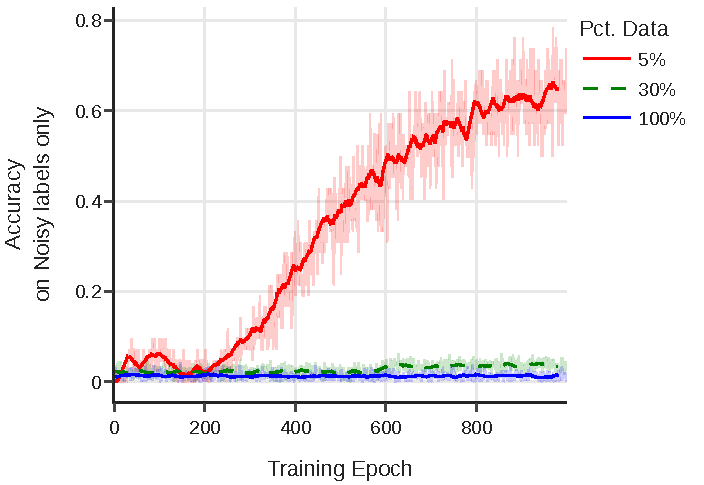
\includegraphics[width=\linewidth]{figures/fig4}
\caption{}
\label{fig:f3_ppa}
\end{subfigure}
\begin{subfigure}{0.45\textwidth}
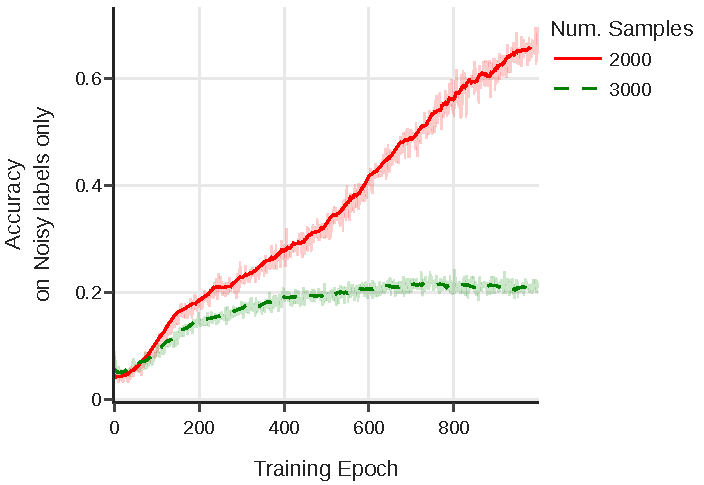
\includegraphics[width=\linewidth]{figures/fig5}
\caption{}
\label{fig:f3_synth}
\end{subfigure}
\caption{Effect of training-set size on noise memorization (training accuracy on noisy labels only). (a) PPA subsampling at $20\%$ symmetric noise. (b) Synthetic graphs of order 7, 6 classes, $35\%$ noise.}
\end{figure}

\section{Dirichlet-Energy Amplification in High-Frequency Components}
\label{app:amplification}
We use the HLFF-GNN framework~\citep{hlffgnn} (implemented as \texttt{FGRLConv}) to decompose representations into low-frequency $Z_1$, high-frequency $Z_2$, and residual $Y$. Under the composite loss
\begin{equation}
\mathcal{L}=\|Y-X\|_F^2+\lambda\,\mathrm{tr}(Z_1^\top\mathbf{\Delta}Z_1)+\alpha\,\mathrm{tr}(Z_2^\top(\mathbf{I}-\mathbf{\Delta})Z_2)+\beta(\|Y^\top Z_1\|_F^2+\|Y^\top Z_2\|_F^2),
\end{equation}
the spectral form of the high-frequency energy is $\Edir(Z_2)=\sum_{r,u}\lambda_u(\bm{\psi}_u^\top Z_{2,r})^2$, in which large $\lambda_u$ amplify any noise-driven content. On ENZYMES with $30\%$ symmetric noise, we observe a sharp monotone increase in $\Edir(Z_2)$, while $\Edir(Z_1)$ and $\Edir(Y)$ remain stable, consistent with Theorem~\ref{thm:noise_forces_energy} and Corollary~\ref{cor:asymmetric}.

\begin{figure}[h]
\centering
\begin{subfigure}{0.45\textwidth}
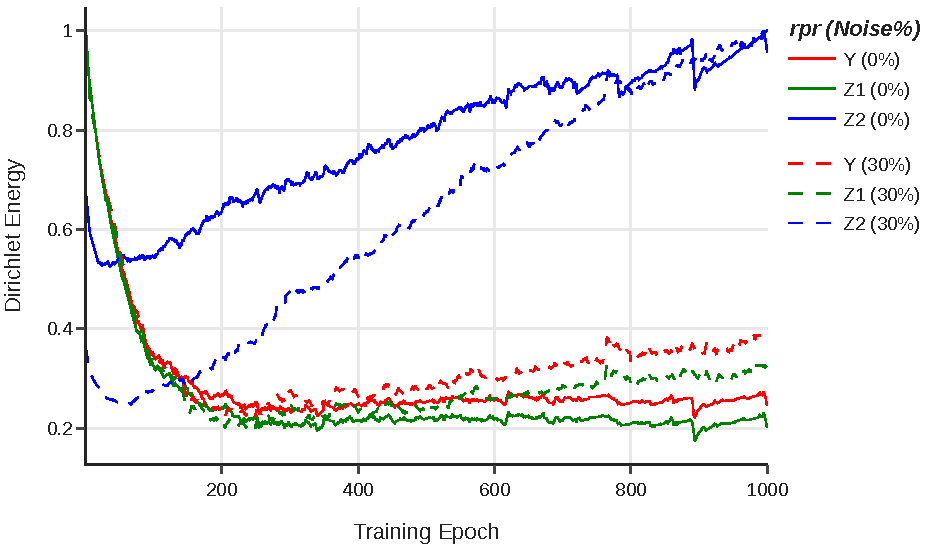
\includegraphics[width=\linewidth]{figures/enzymez1z2y.pdf}
\caption{Normalized $\Edir(Y,Z_1,Z_2)$.}
\end{subfigure}
\hfill
\begin{subfigure}{0.45\textwidth}
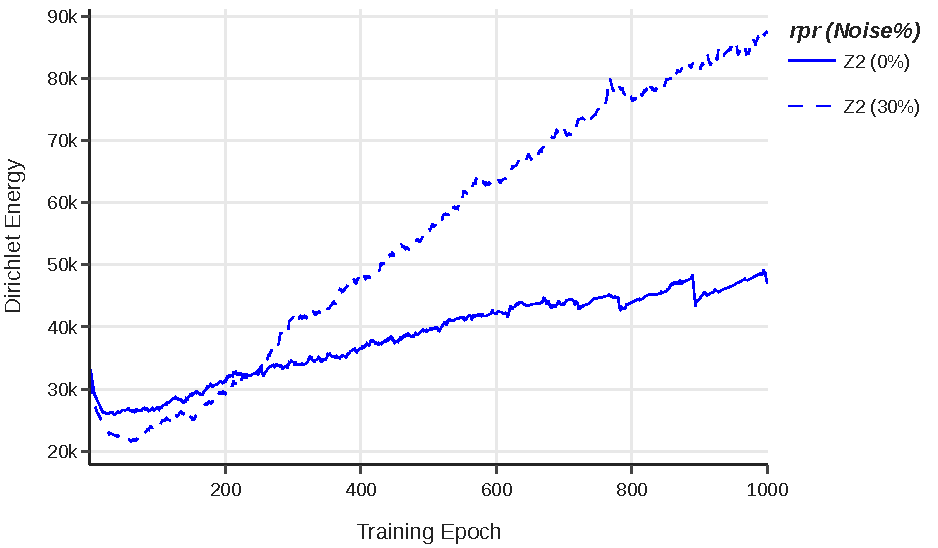
\includegraphics[width=\linewidth]{figures/enzymez2.pdf}
\caption{$\Edir(Z_2)$ alone.}
\end{subfigure}
\caption{HLFF-GNN frequency decomposition on ENZYMES. Solid lines: clean labels. Dashed: $30\%$ symmetric noise. The high-frequency component $Z_2$ is the only one whose energy diverges under noise, supporting the theoretical prediction.}
\label{fig:amplification}
\end{figure}

\section{Additional Empirical Studies on Energy Behavior}
\label{app:additional_studies}

\textbf{Energy under clean overfitting vs.\ noise.} On ENZYMES without regularization, a deliberately overfit GIN exhibits rising training accuracy and rising $\Edirset$, confirming that energy tracks overfitting in general. However, the rise under noise is markedly steeper.

\textbf{Energy scales with noise rate.} On the controlled PPA subset, we sweep symmetric noise $\in\{10,20,30,40,60\}\%$. All curves follow the same U-shape (initial decrease, then rise), and the asymptotic energy increases monotonically with noise rate. This monotonicity is what makes $\Edirset$ a diagnostic.

\begin{figure}[h]
\centering
\begin{subfigure}{0.45\textwidth}
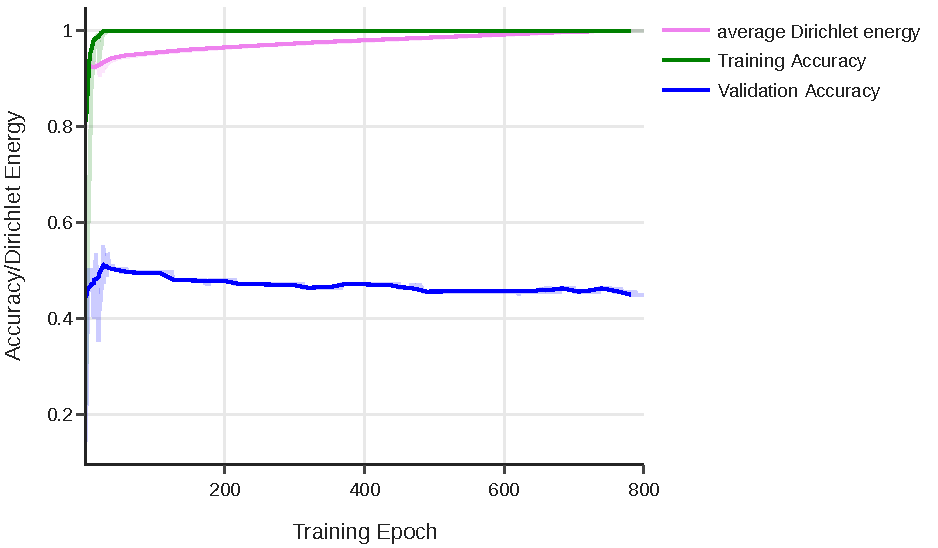
\includegraphics[width=\linewidth]{figures/overfit_enzyme.pdf}
\caption{Clean overfitting on ENZYMES.}
\label{fig:enzymes_energy}
\end{subfigure}
\hfill
\begin{subfigure}{0.45\textwidth}
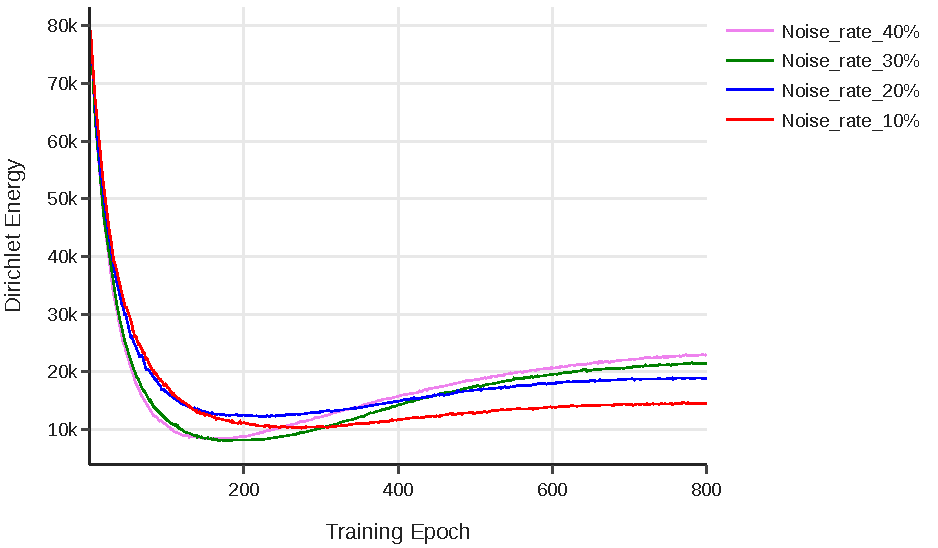
\includegraphics[width=\linewidth]{figures/ablation_noise.pdf}
\caption{$\Edirset$ vs.\ noise rate on PPA.}
\label{fig:noise_levels_energy}
\end{subfigure}
\caption{(a) Even without label noise, energy rises during overfitting; the surge under noise is much steeper. (b) Higher noise rates yield monotonically higher final energy.}
\end{figure}

\section{Additional Tables and Figures}
\label{app:additional_tables}

\begin{table}[h]
\centering
\caption{Sensitivity of \method{} to the learning rate $\eta_u$ of the outlier parameter $\mathbf{u}$, under $40\%$ asymmetric noise.}
\label{tab:lr_sensitivity}
\begin{tabular}{lccc}
\toprule
\textbf{Dataset} & $\eta_u=1$ & $\eta_u=0.1$ & \% Change\\
\midrule
PROTEINS & $76.19$ & $75.89$ & $-0.39\%$\\
MNIST    & $72.61$ & $72.48$ & $-0.18\%$\\
ENZYMES  & $69.81$ & $68.33$ & $-2.12\%$\\
IMDB-B   & $72.89$ & $71.94$ & $-1.30\%$\\
MUTAG    & $93.19$ & $92.61$ & $-0.62\%$\\
REDDIT   & $47.94$ & $48.08$ & $+0.29\%$\\
MSRC-21  & $95.57$ & $95.45$ & $-0.13\%$\\
\bottomrule
\end{tabular}
\end{table}

\begin{table}[h]
\centering
\caption{Performance of CE vs.\ \method{} with $20\%$ symmetric label noise. Last column reports the absolute gain (\method{}$-$CE) on test accuracy.}
\label{tab:alldataset}
\resizebox{0.6\linewidth}{!}{
\begin{tabular}{llcccc}
\toprule
\textbf{Dataset} & \textbf{Metric} & \textbf{0\% CE} & \textbf{20\% CE} & \textbf{20\% \method{}} & \makecell[c]{\textbf{20\%}\\(\method{}$-$CE)}\\
\midrule
\multirow{3}{*}{MNIST}    & Best & $72.69$ & $66.30$ & $71.26$ & $+4.96$\\
                          & Last & $69.80$ & $53.64$ & $67.88$ & $+14.24$\\\cline{3-5}
                          & Diff & $2.89$  & $12.66$ & $3.38$  &\\
\midrule
\multirow{3}{*}{ENZYMES}  & Best & $73.33$ & $64.16$ & $68.69$ & $+4.53$\\
                          & Last & $65.78$ & $57.50$ & $62.54$ & $+5.04$\\\cline{3-5}
                          & Diff & $7.55$  & $6.66$  & $6.15$  &\\
\midrule
\multirow{3}{*}{MSRC-21}  & Best & $96.69$ & $90.26$ & $94.69$ & $+4.43$\\
                          & Last & $93.80$ & $79.64$ & $90.26$ & $+10.62$\\\cline{3-5}
                          & Diff & $2.89$  & $10.62$ & $4.43$  &\\
\midrule
\multirow{3}{*}{PROTEINS} & Best & $81.16$ & $76.23$ & $79.38$ & $+3.15$\\
                          & Last & $79.18$ & $62.32$ & $78.12$ & $+15.80$\\\cline{3-5}
                          & Diff & $1.98$  & $13.91$ & $1.26$  &\\
\midrule
\multirow{3}{*}{MUTAG}    & Best & $94.73$ & $89.47$ & $90.01$ & $+0.54$\\
                          & Last & $84.21$ & $68.42$ & $86.84$ & $+18.42$\\\cline{3-5}
                          & Diff & $10.52$ & $21.05$ & $3.17$  &\\
\midrule
\multirow{3}{*}{IMDB-B}   & Best & $76.50$ & $75.00$ & $75.40$ & $+0.40$\\
                          & Last & $71.60$ & $71.00$ & $73.50$ & $+2.50$\\\cline{3-5}
                          & Diff & $4.90$  & $4.00$  & $1.90$  &\\
\midrule
\multirow{3}{*}{REDDIT}   & Best & $48.15$ & $45.05$ & $44.98$ & $-0.07$\\
                          & Last & $46.01$ & $44.67$ & $44.89$ & $+0.22$\\\cline{3-5}
                          & Diff & $2.14$  & $0.38$  & $0.09$  &\\
\bottomrule
\end{tabular}}
\end{table}

\begin{figure}[h]
\centering
\begin{subfigure}{0.45\textwidth}
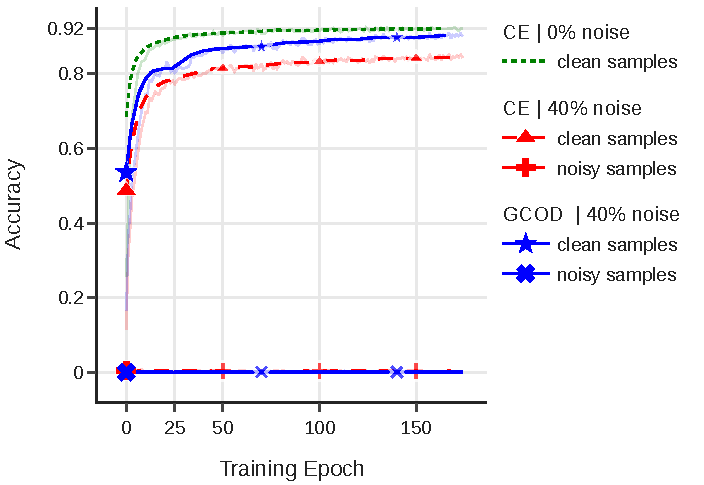
\includegraphics[width=\linewidth]{figures/fig1a.pdf}
\caption{}
\label{fig:noisy_pure_40_1}
\end{subfigure}
\begin{subfigure}{0.45\textwidth}
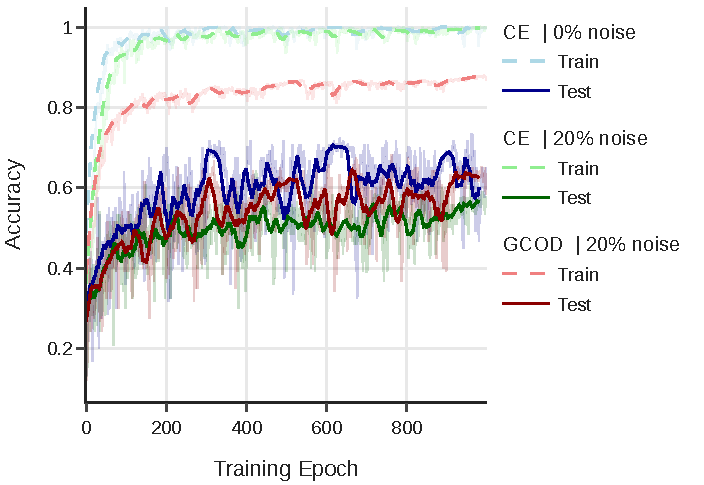
\includegraphics[width=\linewidth]{figures/fig6}
\caption{}
\label{fig:gin_enzymes}
\end{subfigure}
\caption{(a) Train accuracy on known noisy and clean PPA subsets (4-class, $40\%$ symmetric noise) for GCN with CE: the model never separates noisy from clean training samples without a robust loss. (b) Train/test accuracy on ENZYMES with GIN under clean and $20\%$ symmetric noise.}
\end{figure}

\begin{figure}[h]
\centering
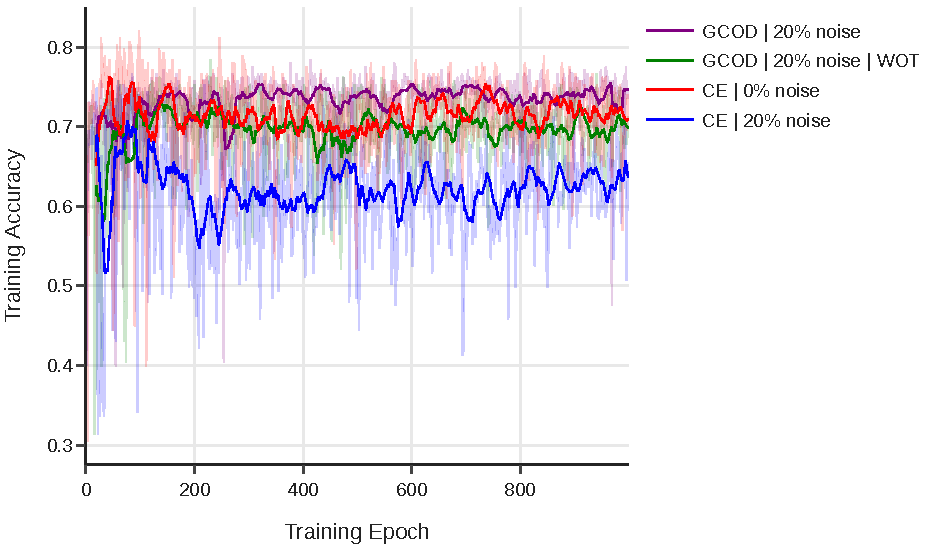
\includegraphics[width=0.45\linewidth]{figures/ablation_trainingacc.pdf}
\caption{Ablation on the training-accuracy feedback in \method{}. Without scaling $u$ by $a_{\text{train}}$ (``GCOD WOT''), the outlier parameter dominates early and harms generalization; the full \method{} activates outlier-discounting gradually.}
\label{fig:uablation}
\end{figure}

\begin{figure}[h]
\centering
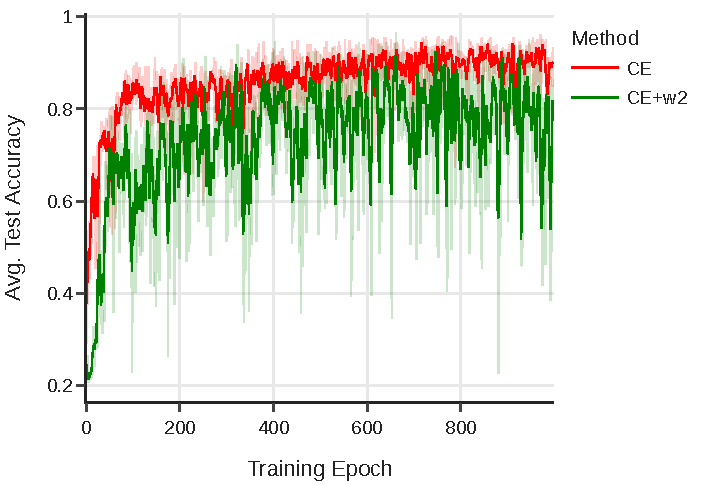
\includegraphics[width=0.45\linewidth]{figures/unstability.pdf}
\caption{Test accuracy on PPA-30\%-6 for CE and CE+W2. CE+W2 reaches comparable peak accuracy but exhibits unstable convergence due to the per-epoch eigendecomposition.}
\label{fig:unstability_app}
\end{figure}

\begin{figure}[h]
\centering
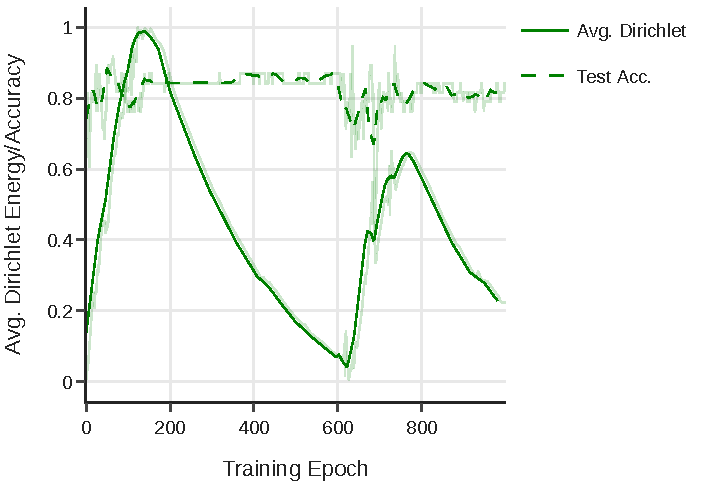
\includegraphics[width=0.45\linewidth]{figures/mutag.pdf}
\caption{Average test accuracy and average within-graph $\Edirset$ on MUTAG ($0\%$ noise) with GIN: classification accuracy improves while energy decays, the clean-data signature of a healthy GNN.}
\label{fig:mutag_app}
\end{figure}

\section{Full ogbg-ppa: Do-No-Harm Check}
\label{app:full_ppa}

The standard ogbg-ppa benchmark has 37 classes and $\sim$158{,}000 graphs of mean order $\approx$240, so a 5-layer GIN with 300 hidden units is structurally \emph{under-parameterized} for the task. We trained CE, $\mathcal{L}_{DE}$ (Fixed), CE+W2 and \method{} on the full benchmark with $0\%$, $20\%$ and $40\%$ symmetric noise. Two qualitative observations are robust across runs:

\begin{enumerate}[leftmargin=*,itemsep=0.5pt,topsep=2pt]
\item \emph{Training accuracy on the noisy-labeled subset stays close to chance for all methods, including standard CE.} The under-parameterized model never reaches a regime where it can memorize the corrupted graph-level labels, consistent with our failure-mode analysis of Section~\ref{sec:failure_modes}: F1 (number of classes), F2 (graph order) and F3 (training-set size) all push the full PPA out of the noise-fitting regime.

\item \emph{Test accuracy of our three methods is statistically indistinguishable from CE} at every noise rate. None of CE+W2, $\mathcal{L}_{DE}$, or \method{} perturbs the underlying training dynamics enough to harm clean generalization, since their corrective signals (negative-eigenvalue projection, energy upper bound, outlier discounting) are only triggered by the high-frequency surge that does not occur on the full PPA.
\end{enumerate}

This is by design: the methods are conditional regularizers, not unconditional smoothers. The take-away is that they impose \emph{no measurable overhead in accuracy} when the underlying network is already noise-robust, while providing substantial protection when over-parameterization, low graph order, or small training sets push the network into the noise-fitting regime (Section~\ref{sec:experiments}, controlled PPA-30\%-6 subset). A fair generality claim therefore rests on the seven additional benchmarks in Tables~\ref{tab:multidataset} and~\ref{tab:alldataset}, with the full PPA serving exclusively as a do-no-harm sanity check.

\section{Cross-Setting Transfer: Cora Node Classification}
\label{app:cora}

To assess whether the energy perspective captures a property of GNN training under label noise that is more general than the graph-classification setting it was designed for, we apply CE+W2 and \method{} \emph{unchanged} to node classification on Cora at $20\%$ symmetric label noise. We use both GAT and GCN backbones, with the standard public split, and compare against $13$ node-classification baselines that include CE, GCE~\citep{ghosh2017robust}, NRGNN~\citep{nrgnn11}, RTGNN~\citep{contrastivelearning5}, GNN-Cleaner, ERASE, CR-GNN, and the standard noise-robust losses adapted to node classification.

\begin{table}[h]
\centering
\caption{Cross-setting transfer of \method{} and CE+W2 to node classification on Cora under $20\%$ symmetric label noise. Numbers are test accuracy; ranks are with respect to the full $13$-method comparison reported in the rebuttal materials. We report only the verified results for our two methods on each backbone; the ``rank'' field indicates their position in the full ranking. The methods are not modified, regularization parameters are kept at their graph-classification defaults.}
\label{tab:cora_transfer}
\renewcommand{\arraystretch}{1.05}
\begin{tabular}{lccc}
\toprule
\textbf{Backbone} & \textbf{Method} & \textbf{Test Acc.} & \textbf{Rank (out of 13)}\\
\midrule
GAT & CE+W2     & $0.8157$ & $\#2$\\
GAT & \method{} & $0.7910$ & $\#4$\\
GCN & \method{} & $0.7403$ & $\#4$\\
GCN & CE+W2     & $0.7247$ & $\#5$\\
\bottomrule
\end{tabular}
\end{table}

Both methods land in the top half of the ranking on each backbone, despite using neither homophily, contrastive losses, pseudo-labels, nor any node-specific machinery. CE+W2 in particular is competitive with the strongest specialized node-classification baselines on GAT. The interpretation, consistent with Theorem~\ref{thm:noise_forces_energy}, is that the spectral mechanism by which noise fitting forces within-graph energy to grow is not specific to graph classification: in node classification, individual labels are also embedded in node-level representations whose Dirichlet energy reflects local smoothness, and constraining that smoothness penalizes the same noise-fitting path. The transfer is therefore not a coincidence but a corollary of the energy-based framing.
